%# -*- coding: utf-8 -*-
\documentclass{ctexart}
%
%页眉页脚

\usepackage{geometry}
\geometry{left=2.5cm,right=2.5cm,top=2.5cm,bottom=2.5cm}

\usepackage{xcolor}
\usepackage{graphicx}
\usepackage{amsmath}
\usepackage{url}
\usepackage{enumerate}
\usepackage{subfigure}
\usepackage{listings} 
\usepackage[colorlinks,linkcolor=black]{hyperref}% 书签
\lstset{numbers=left, %设置行号位置
    numberstyle=\tiny, %设置行号大小
    keywordstyle=\color{blue}, %设置关键字颜色
    commentstyle=\color[cmyk]{1,0,1,0}, %设置注释颜色
    frame=single, %设置边框格式
    breaklines, %自动折行
    extendedchars=false, %解决代码跨页时,章节标题,页眉等汉字不显示的问题
    xleftmargin=1.5em,xrightmargin=1.5em, aboveskip=1em, %设置边距
    tabsize=4, %设置tab空格数
    showspaces=false %不显示空格
}
%中文
\usepackage{xeCJK}
%字体设置
\usepackage{indentfirst}
\setlength{\parindent}{2em} %首行缩进



\title{MATLAB 综合实验之语音合成\footnote{所有的.m文件均采用utf8编码,在matlab中打开可能会出现中文乱码的情况,请用其它编辑器打开}}
\author{聂浩~~ 无31~~ 2013011280}
\date{\today}
\begin{document}
\maketitle
\section{语音预测模型}
\subsection{
    给定$e(n) = s(n)-a_1s(n-1)-a2_s(n-2)$假设 e(n) 是输入信号,s(n)
    是输出信号,上述滤波器的传递函数是什么?如果 $a_1 = 1.3789,
    a_2 =-0.9506$ ,上述合成模型的共振峰频率是多少?用 zplane ,
    freqz ,impz 分别绘出零 极点图,频率响应和单位样值响应。
用 filter 绘出单位样值响应,比较和 impz 的是否相同。}

答:传递函数是

\[V(s)=\frac{1}{1-a_1z^{-1}-a_2z^{-2}}=\frac{1}{1-1.3789z^{-1}+0.9506z^{-2}}\]

共振峰频率为\[f=\frac{\Omega}{2\pi T}=999.947Hz\].

zplane绘制零极点图如图\ref{1zp},freqz绘制频率响应图如图\ref{1freq},impz和filter绘制单位样值响应如图\ref{1ir}.

从图中可以看出,impz和filter绘制的图像是一致的。

\begin{figure}
    \centering
    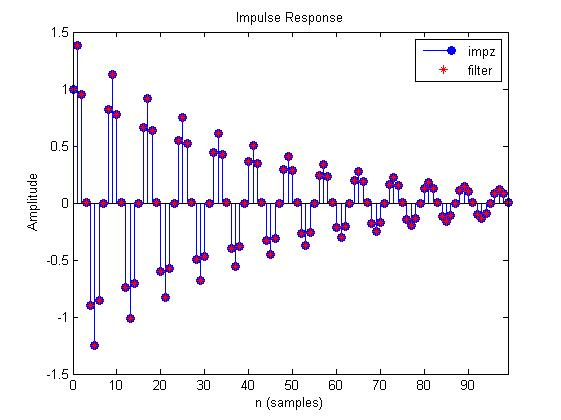
\includegraphics[width=0.8\textwidth]{1_zp.jpg}\\
    \caption{零极点图\label{1zp}}
\end{figure}

\begin{figure}
    \centering
    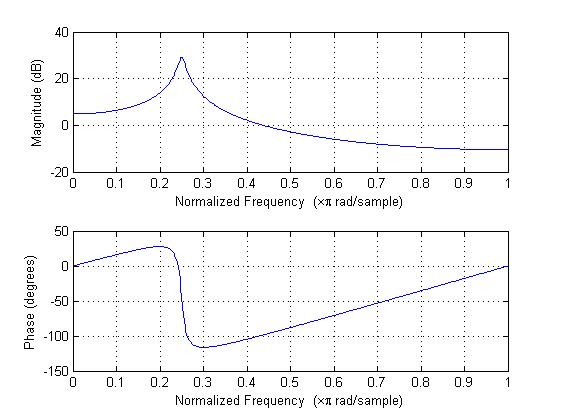
\includegraphics[width=0.8\textwidth]{1_freqz.jpg}\\
    \caption{频率响应图\label{1freq}}
\end{figure}

\begin{figure}
    \centering
    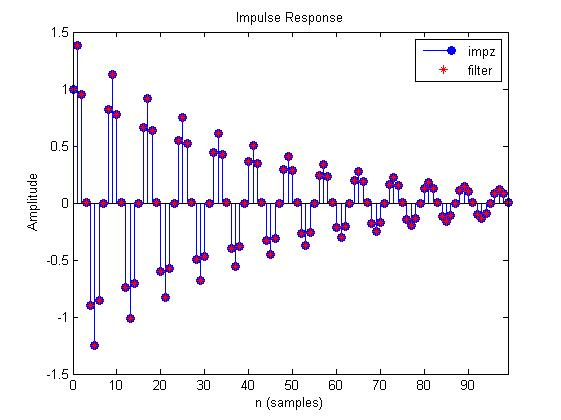
\includegraphics[width=0.8\textwidth]{1_zp.jpg}\\
    \caption{单位样值响应图\label{lir}}
\end{figure}

代码如下(a21.m):
\lstinputlisting[language=matlab]{a21.m}

\subsection{
    阅读 speechproc.m 程序,理解基本流程。程序中已经完成了语音分帧、加窗、线
    性预测、和基音周期提取等功能。注意:不要求掌握线性预测和基音周期提取的算法原理。
}

以8KHz的采样频率,10ms(80个点)为一段,对从第三段起的每一段用haming窗加窗后进行处理。
\subsection{
运行该程序到 27 帧时停住,用(1)中的方法观察零极点图。 }

零极点图如图\ref{2zp}
\begin{figure}
    \centering
    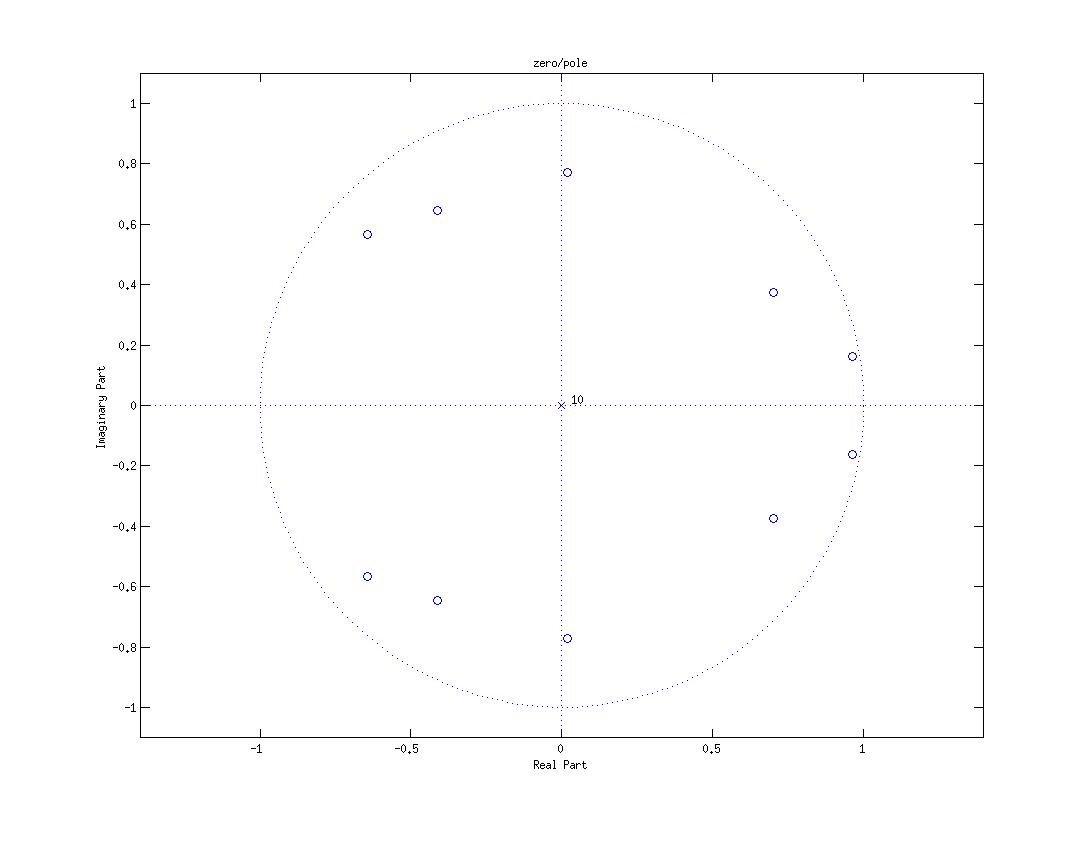
\includegraphics[width=0.8\textwidth]{2_zp.jpg}\\
    \caption{单位样值响应图\label{2zp}}
\end{figure}

代码如下:
\begin{lstlisting}[language=matlab]
if n == 27
% (3) 在此位置写程序,观察预测系统的零极点图
zplane(A)
title('zero/pole'); 
end
\end{lstlisting}

\subsection{
    在循环中添加程序:对每帧语音信号 s(n) 和预测模型系数\{$a_i$\},用 filter 计算 激励信号 e(n) 。注意:在系数变化的情况下连续滤波,需维持滤波器的状态不变,要利用
    filter 的 zi 和 zf 参数。
}
代码如下:
\begin{lstlisting}[language=matlab]
s_f = s((n-1)*FL+1:n*FL);       
% 本帧语音,下面就要对它做处理
% (4) 在此位置写程序,用filter 函数 s_f  计算激励,注意保持滤波器状态
% exc((n-1)*FL+1:n*FL) = ...  将你计算得到的激励写在这里
[exc((n-1)*FL+1:n*FL),zi_pre]=filter(A,1,s_f,zi_pre);
\end{lstlisting}

\subsection{
完善 speechproc.m 程序,在循环中添加程序:用你计算得到的激励信号 e(n) 和预 测模型系数\{$a_i$\},用 filter 计算重建语音 $\hat{s}(n)$ 。同样要注意维持滤波器的状态不变。 }

这里需要反过来用滤波器,代码如下:
\begin{lstlisting}[language=matlab]
% (5) 在此位置写程序,用filter 函数
%和exc 重建语音,注意保持滤波器状态
[s_rec((n-1)*FL+1:n*FL),zi_rec]=filter(1,A,exc((n-1)*FL+1:n*FL),zi_rec);
% s_rec((n-1)*FL+1:n*FL) = ... 将你计算得到的重建语音写在这里
\end{lstlisting}
\subsection{
    在循环结束后添加程序:用 sound 试听(6)中的 e(n) 信号,比较和 s(n) 以及 
$\hat{s}(n)$信号有何区别。对比画出三个信号,选择一小段,看看有何区别}

答:
s(n)和$\hat{s}(n)$无法从听力上区分,e(n)听起来声音比较嘈杂,这是e(n)中的随机噪声所产生的影响。\footnote{$e(n)=s(n)-\sum_{k=1}^{N}a_ks(n-k)$为残差
,由于差分的影响,e(n)与s(n)之间的差是不断变化的}。但仍能从e(n)中分辨出语音内容,可见e(n)中还是保留了不少s(n)的信息。

从波形图图\ref{6wave}可以看出,除了开始和结束两个小节,s(n)和$\hat{s}(n)$是一致的,而e(n)比s(n)要差不少且波形并不一致。从0.2到0.3s的局部波形图\ref{6detail}也可以得出这样的结论。
\begin{figure}
    \centering
    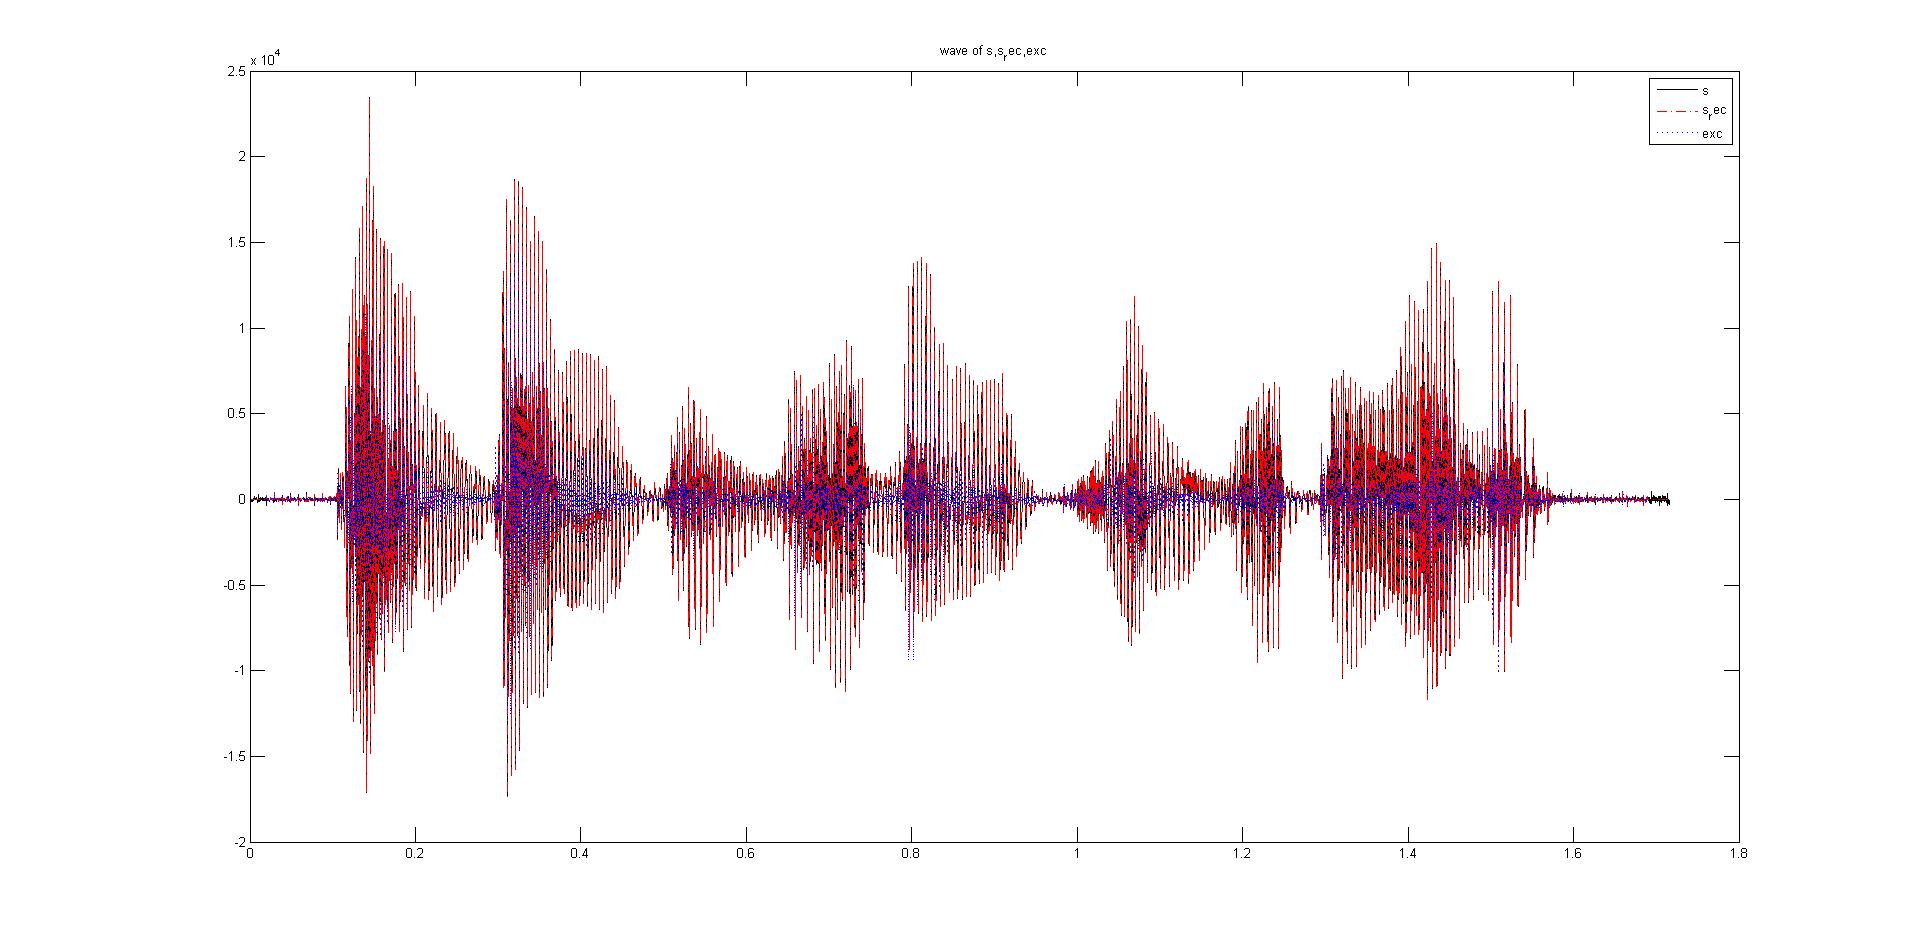
\includegraphics[width=0.8\textwidth]{6_wave.jpg}\\
    \caption{波形图\label{6wave}}
\end{figure}


\begin{figure}
    \centering
    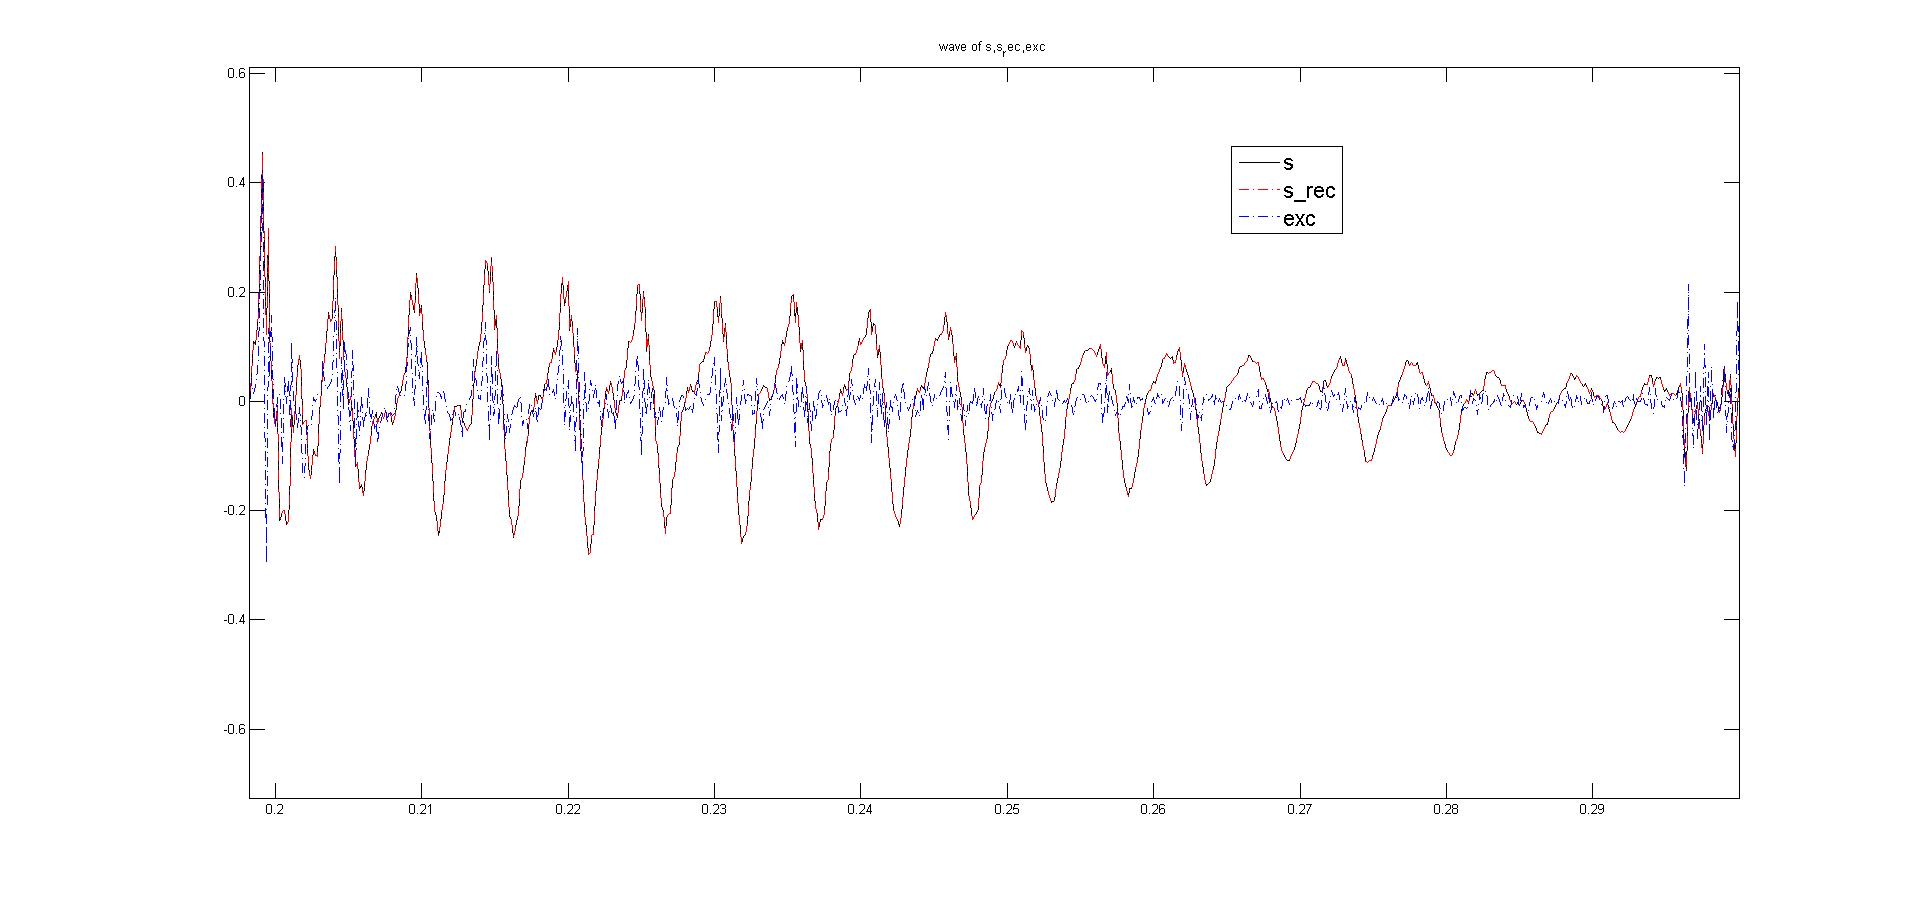
\includegraphics[width=0.8\textwidth]{6_detail.jpg}\\
    \caption{0.2到0.3s波形图\label{6detail}}
\end{figure}


\section{
语音合成模型
}
\setcounter{subsection}{6} 

\subsection{
生成一个 8kHz 抽样持续 1 秒钟的数字信号,该信号是一个频率为 200Hz 的单
位样值“串”,即
$x(n)=\sum_{i=0}^{NS-1}\delta(n-iN)$
考虑该信号的 N 和 NS 分别为何值?用 sound 试听这个声音信号。再生成一个 300Hz 的单
位样值“串”并试听,有何区别?事实上,这个信号将是后面要用到的以基音为周期的人工
激励信号 e(n) 。
}

答:NS应当为200,N应为40。300Hz的音听起来音调要高一些。和之前音乐合成的正弦波相比,这两个音要更尖锐一些。

代码如下(g200.m):
\lstinputlisting[language=matlab]{g200.m}
\subsection{
真实语音信号的基音周期总是随着时间变化的。我们首先将信号分成若干个 10
毫秒长的段,假设每个段内基音周期固定不变,但段和段之间则不同,具体为
$PT = 80 + 5mod(m,50)$
其中 PT 表示基音周期,m 表示段序号。生成 1 秒钟的上述信号并试听。 (提示:用循环逐
段实现,控制相邻两个脉冲的间隔为其中某个脉冲所在段的PT值。 )
}
生成的波形如图\ref{8wave},听起来像是撕布声。

代码如下:
\lstinputlisting[language=matlab]{c_g_8.m}

\begin{figure}
    \centering
    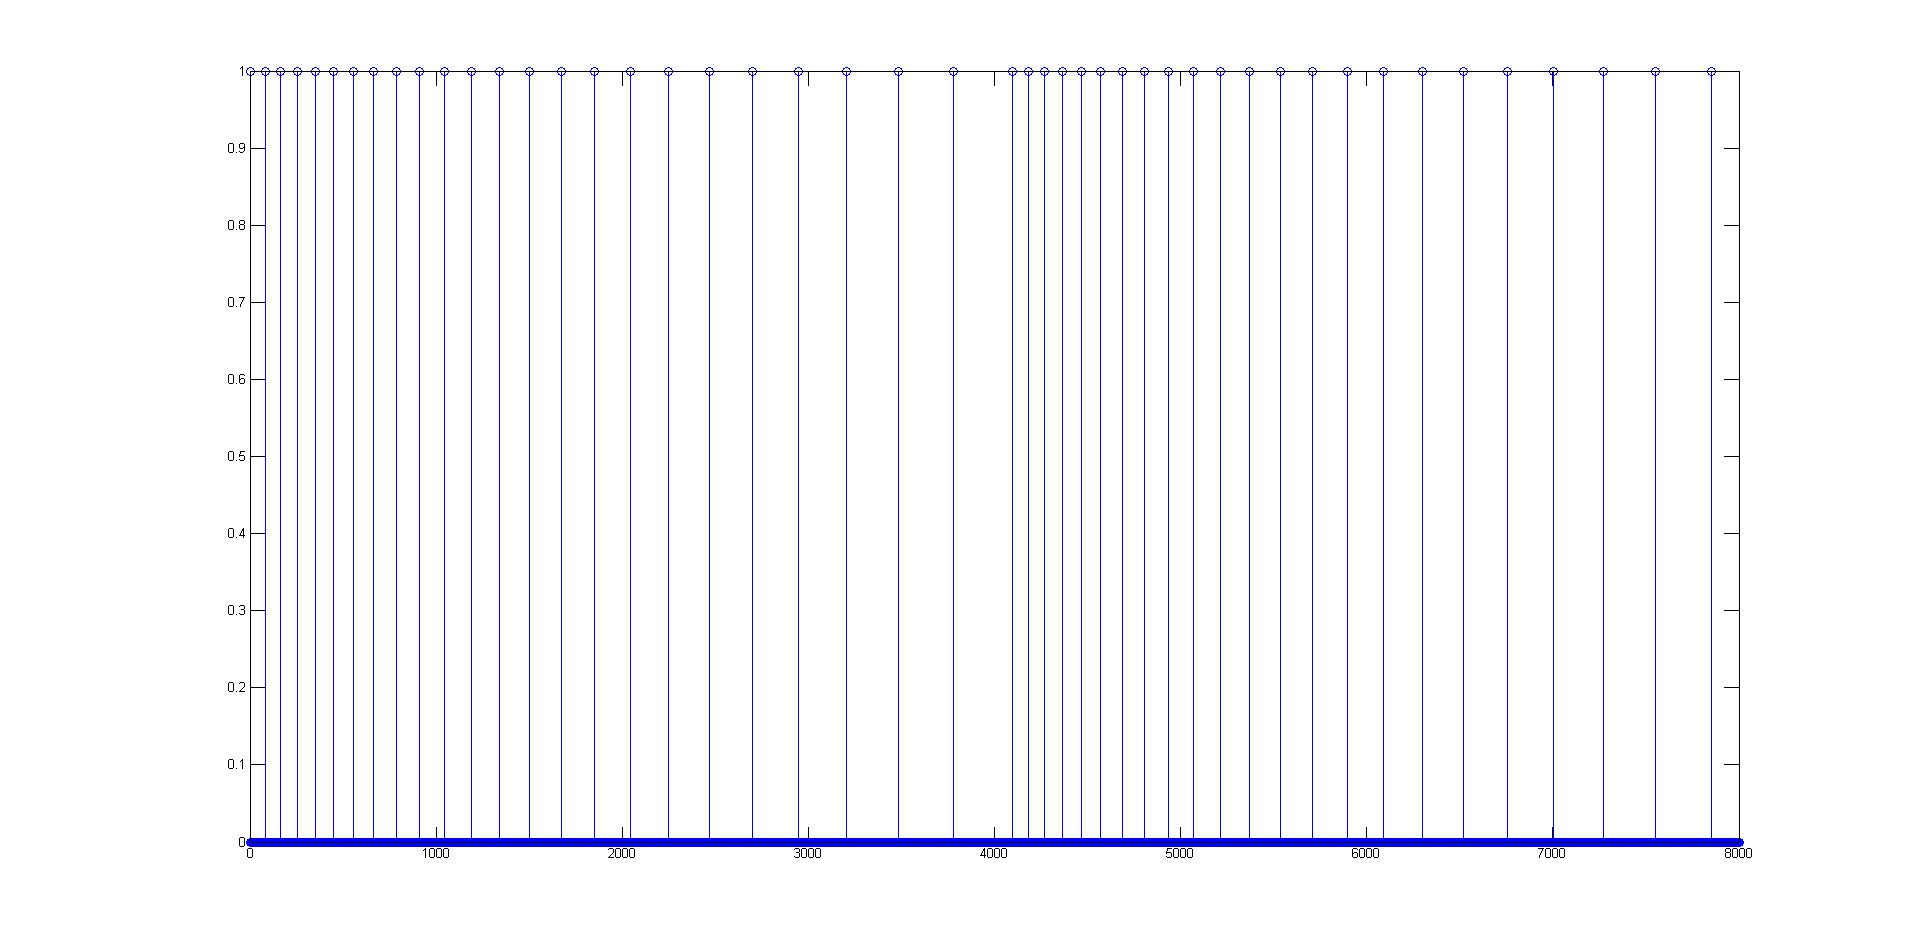
\includegraphics[width=0.8\textwidth]{8wave.jpg}\\
    \caption{生成的e(n)\label{8wave}}
\end{figure}

\subsection{
用 filter 将(8)中的激励信号 e(n) 输入到(1)的系统中计算输出 s(n) ,试听和
e(n) 有何区别。
}

这里听起来就像是给8中的e(n)信号加了一些混响,有一种在e(n)在盒子中发声的感觉,波形如图\ref{9wave}。

代码如下
\lstinputlisting[language=matlab]{c_g_9.m}

\begin{figure}
    \centering
    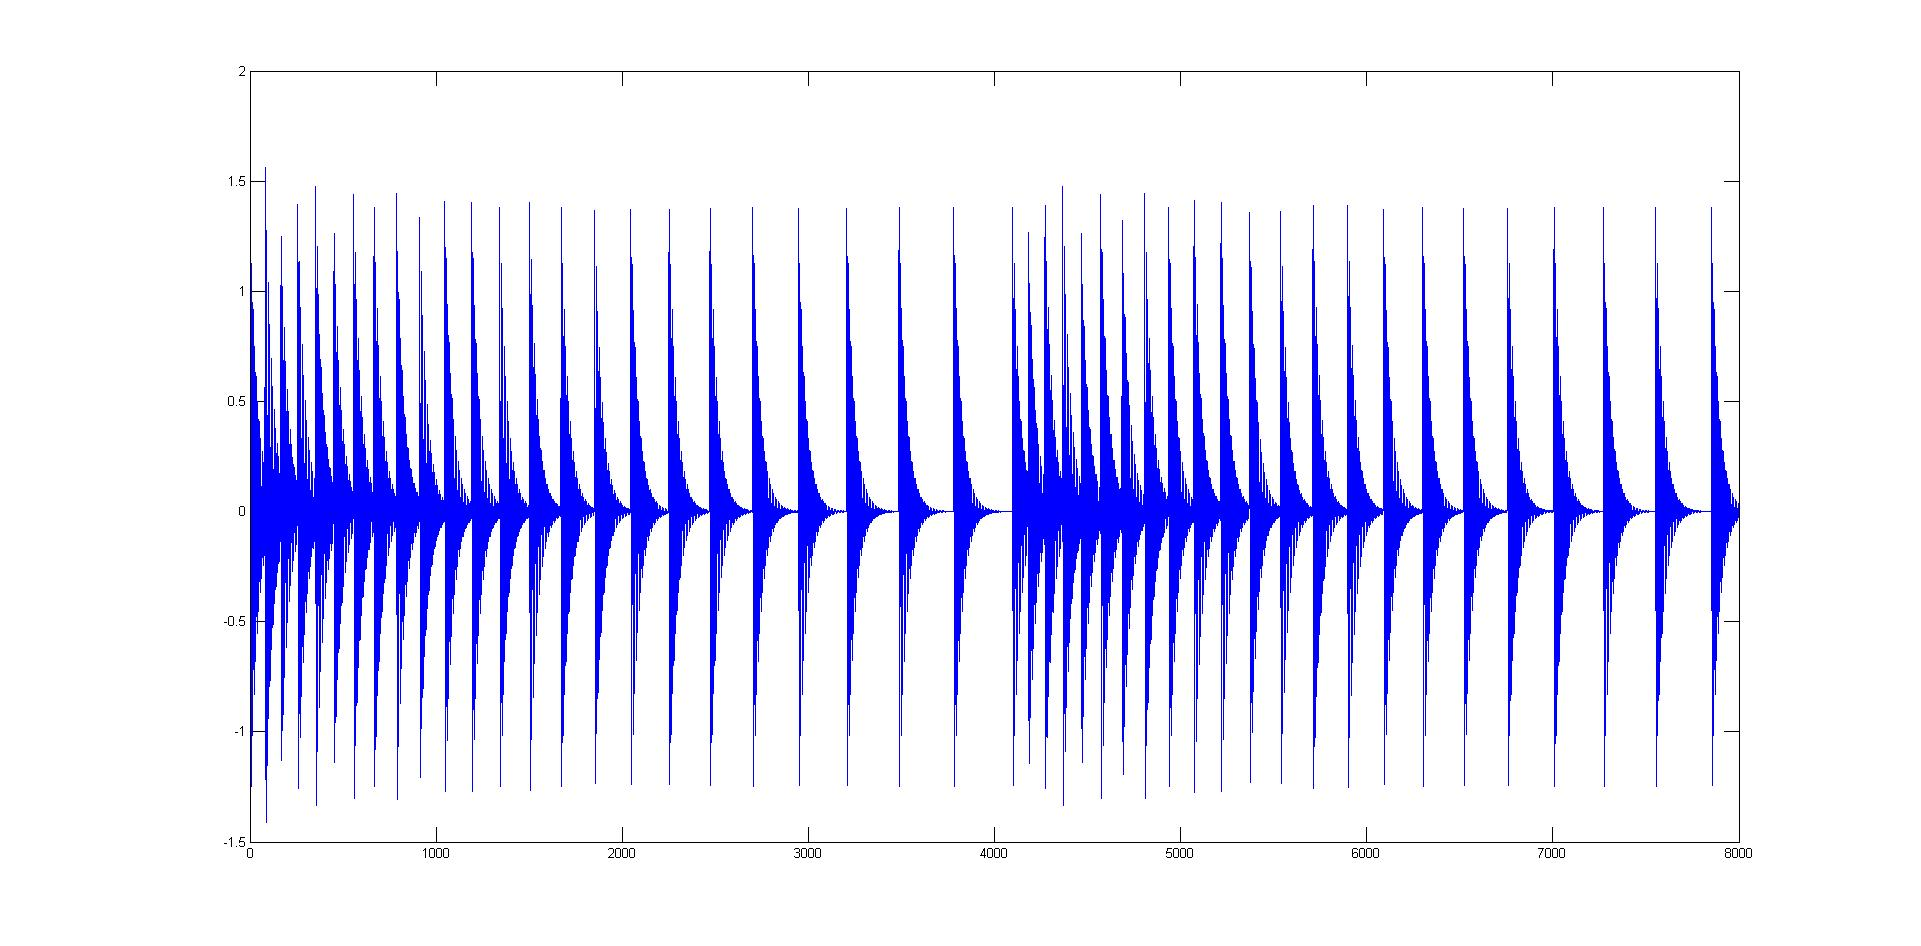
\includegraphics[width=0.8\textwidth]{9wave.jpg}\\
    \caption{处理生成的s(n)\label{9wave}}
\end{figure}

\subsection{
重改 speechproc.m 程序。利用每一帧已经计算得到的基音周期和(8)的方法,
生成合成激励信号 Gx(n)(G 是增益),用 filter 函数将 Gx(n) 送入合成滤波器得到合成语
音 $\tilde{s}(n)$ 。试听和原始语音有何差别。
}
这里的的$\tilde{s}(n)$听起来在每两个字之间有一种模糊的感觉,就像风吹在麦克风上一样。
这应该是因为基频在这些时刻快速改变造成的。

代码如下:
\begin{lstlisting}[language=matlab]
% (10) 在此位置写程序,生成合成激励,并用激励和filter 函数产生合成语音

% exc_syn((n-1)*FL+1:n*FL) = ... 将你计算得到的合成激励写在这里
tmp=(n-1)*FL+1:n*FL;
exc_syn((n-1)*FL+1:n*FL)= G*(mod(tmp,PT)==0);

% s_syn((n-1)*FL+1:n*FL) = ...   将你计算得到的合成语音写在这里
[s_syn((n-1)*FL+1:n*FL),zi_syn]=filter(1,A,exc_syn((n-1)*FL+1:n*FL),zi_syn);
\end{lstlisting}

在最前部还应该加上zi\_syn的定义
\begin{lstlisting}[language=matlab]
zi_syn = zeros(P,1);
\end{lstlisting}

\section{变速不变调}
\setcounter{subsection}{10} 

\subsection{
仿照(10)重改 speechproc.m 程序,只不过将(10)中合成激励的长度增加一倍,
即原来 10 毫秒的一帧变成了 20 毫秒一帧,再用同样的方法合成出语音来,如果你用原始
抽样速度进行播放,就会听到慢了一倍的语音,但是音调基本没有变化。
}    
这样的到的语音长为原来的两倍,但是音调并未变化,这与直接慢放(resample增加采样点)的结果完全不一样。
代码如下:
\begin{lstlisting}[language=matlab]
% (11) 不改变基音周期和预测系数,将合成激励的长度增加一倍,再作为filter
% 的输入得到新的合成语音,听一听是不是速度变慢了,但音调没有变。
tmp_syn_v=(n-1)*FL_v+1:n*FL_v;
% exc_syn_v((n-1)*FL_v+1:n*FL_v) = ... 将你计算得到的加长合成激励写在这里
exc_syn_v((n-1)*FL_v+1:n*FL_v)= G*(mod(tmp_syn_v,PT)==0);
% s_syn_v((n-1)*FL_v+1:n*FL_v) = ...   将你计算得到的加长合成语音写在这里
[s_syn_v((n-1)*FL_v+1:n*FL_v),zi_syn_v]=filter(1,A,exc_syn_v((n-1)*FL_v+1:n*FL_v),zi_syn_v);
\end{lstlisting}

在最前部还应该加上FL\_v和zi\_syn\_v的定义
\begin{lstlisting}[language=matlab]
FL_v=2*FL;
zi_syn_v = zeros(P,1);
\end{lstlisting}
\section{变调不变速}
\setcounter{subsection}{11} 

\subsection{
重新考察(1)中的系统,将其共振峰频率提高 150Hz 后的 a1 和 a2 分别是多少?
}
\[a_1=1.2073,a_2=-0.9506\]

代码如下:
\lstinputlisting[language=matlab]{a212.m}

\subsection{
仿照(10)重改 speechproc.m 程序,但要将基音周期减小一半,将所有的共振峰
频率都增加 150Hz ,重新合成语音,听听是何感受。
}
听起来调子高了不少,但音频时长并未改变。然而并不是非常像女声,有很强的假声的感觉。

代码如下:
\begin{lstlisting}[language=matlab]
% (13) 将基音周期减小一半,将共振峰频率增加150Hz,重新合成语音,听听是啥感受~
PT=fix(PT/2);
[z,p,k]=tf2zp(1,A);
%角度为正频率加155
%为负减155
p=abs(p).*exp((  angle(p)+2*pi/8000*150*  (2* (angle(p)>0) -1)  )*1j);
[B,A]=zp2tf(z,p,k);
tmp_t=(n-1)*FL+1:n*FL;
% exc_syn_t((n-1)*FL+1:n*FL) = ... 将你计算得到的变调合成激励写在这里
exc_syn_t((n-1)*FL+1:n*FL)= G*(mod(tmp_t,PT)==0);
% s_syn_t((n-1)*FL+1:n*FL) = ...   将你计算得到的变调合成语音写在这里
[s_syn_t((n-1)*FL+1:n*FL),zi_syn_t]=filter(B,A,exc_syn_t((n-1)*FL+1:n*FL),zi_syn_t);
\end{lstlisting}

在最前部还应该加上zi\_syn\_t的定义
\begin{lstlisting}[language=matlab]
zi_syn_t = zeros(P,1);
\end{lstlisting}

\section{总结}
本次试验更多的是利用已有的数学模型在给定框架下进行扩展,与音乐合成实验相比发散性更少一些,最终的实现也较为单一。感觉本次实验最大的收获是对于语音合成、语音处理的进一步理解,matlab更多的是应用。

\section{speechproc.m完成版}
\lstinputlisting[language=matlab]{speechproc.m}

\end{document}
